\documentclass[../Main.tex]{subfiles}

\begin{document}
\author{Circuits} %use author for title of lesson
\date{Year 1 Topic 14} %use date to refer to topic in main booklet

\section{Circuits} %Section is the title of the lesson repeated, ready for the main contents page.

\begin{frame}{Series Circuit}
    Cast your mind back to GCSE... what could you tell me about a series circuit in terms of current, voltage, and resistance?
    \begin{figure}
        \centering
        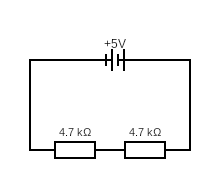
\includegraphics[height=3cm]{Electricity_Images/series_circuit.png}
    \end{figure} \pause

      \begin{block}{Important to remember!}
    \begin{itemize}
        \item Current is the same always
        \item Voltage is split across components
        \item Total resistance is added up
    \end{itemize}
    \begin{equation*}
        I_1=I_2=I_3 \hspace{1cm} \varepsilon = V_1 + V_2 \hspace{1cm}  R_T=R_1+R_2
    \end{equation*}
    \end{block}
\end{frame}

\begin{frame}{Kirchhoff's 2nd Law}
    \begin{block}{K2L}
    Kirchhoff's second law states that, for a closed loop, the sum of the e.m.fs is equal to the sum of the p.ds
    
    \begin{equation*}
        \Sigma \varepsilon = \Sigma V
    \end{equation*}
    \end{block}
    
    \begin{figure}
        \centering
        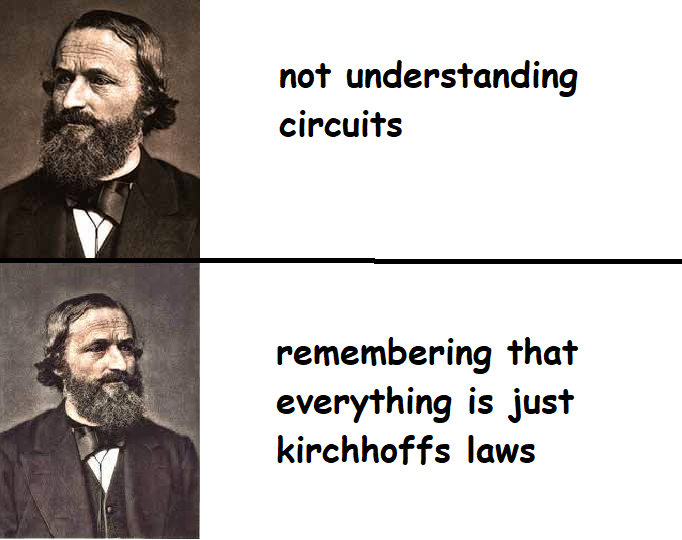
\includegraphics[height=4cm]{Electricity_Images/kirchoffs_laws_meme.png}
    \end{figure}
\end{frame}

\begin{frame}{Potential Divider}
    A potential divider is a circuit designed to produce a determined output voltage lower than the supply voltage for subsequent use. This circuit is usually a combination of resistors. 
    \newline
    \pause
    \newline
   We know the voltage across a resistor is proportional to the resistance ($V\propto R$ -- ohm's law). Now if we imagine two resistors in series, where one is double the other, the total emf is split across them in a 2:1 ratio. 
   
   \begin{equation*}
       \frac{V_1}{V_2} = \frac{R_1}{R_2}
   \end{equation*}
   
   This leads to us being able to easily calculate the voltage across the resistors if we know one of them. 
\end{frame}

\begin{frame}{Potential Divider}
    But what if we don't know the voltage across either of the resistors?
    \pause
     \begin{equation*}
        V_{out} = \frac{V_{in}R_2}{R_1+R_2}
    \end{equation*}
    This is the potential divider formula. From it, we take $V_{out}$ to be the voltage across the second resistor - but how could we find the resistance across the first resistor?
  
    \begin{exampleblock}{Example}
    A potential divider has two resistors $R_1=40 \Omega \mbox{ and } R_2=60 \Omega$. With an input voltage of 5V, determine the output voltage of the potential divider. \pause
    --3V
\end{exampleblock} \pause

\begin{exampleblock}{Example 2 - your turn}
    For the same potential divider, calculate the output voltage across $R_1$. \pause
    --2V 
\end{exampleblock}
\end{frame}

\begin{frame}{Potential Divider}
    \begin{exampleblock}{You Try!}
        (These are Kerboodle questions -- section 10.5, you can find the answers at the back of the book)
        
        \begin{figure}
            \centering
            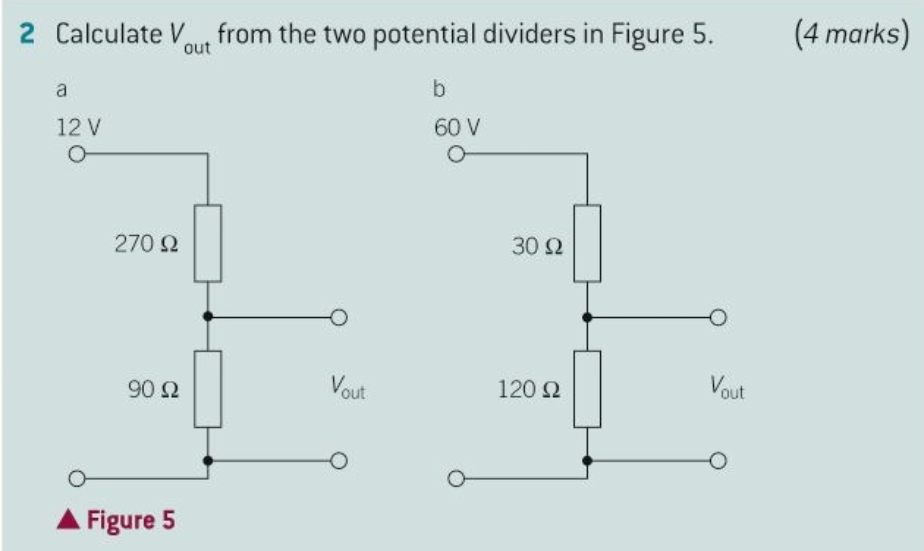
\includegraphics[height=4cm]{Electricity_Images/potential_divider_questions.jpg}
        \end{figure}
    \end{exampleblock}
\end{frame}

\begin{frame}{Current in a series circuit}
    How might we find the total current in a series circuit? \pause
    \newline \newline
    For a circuit, we know V=IR. This means that if we know the total resistance of all the components, and the emf supplied from the power supply, we can work out the current very easily. 
   
    \begin{block}{Total resistance}
    In series, resistance adds up: $R_T= \Sigma R$
    \end{block}
    
    So what would the total resistance, and hence the current, of this circuit be?
    
    \begin{figure}
        \centering
        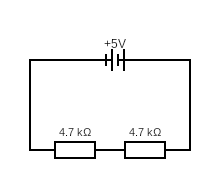
\includegraphics[height=3cm]{Electricity_Images/series_circuit.png}
    \end{figure}
\end{frame}

\begin{frame}{Parallel Circuits}
    Okay, so what about parallel circuits? Cast your mind back to GCSE - what could you tell me in terms of voltage, current, and resistance?
    
    \begin{figure}
        \centering
        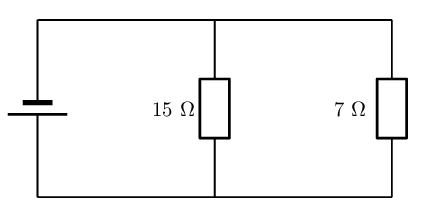
\includegraphics[height=3cm]{Electricity_Images/parallel_circuit.png}
    \end{figure} \pause
    
       \begin{block}{Important to remember!}
    \begin{itemize}
        \item Current is split across branches (Kirchhoff's first law)
        \item Voltage is the same across branches
    \end{itemize}
    
    \begin{equation*}
        I=I_1+I_2 \hspace{1cm} \varepsilon = V_1 = V_2 
    \end{equation*}
    \end{block}
\end{frame}

\begin{frame}{Resistors in parallel}
    When finding the overall resistance in parallel, things are a bit different... 
    
    \begin{equation*}
        \frac{1}{R_T}=\frac{1}{R_1}+\frac{1}{R_2}+... \pause 
        = \sum \frac{1}{R}
    \end{equation*}

\begin{figure}
    \centering
    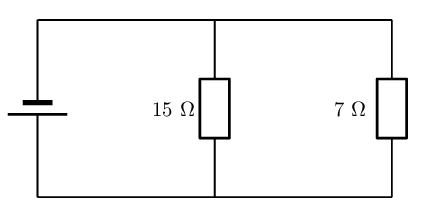
\includegraphics[height=4cm]{Electricity_Images/parallel_circuit.png}
\end{figure}

Alternatively, for just 2 resistors in parallel: $R=\frac{R_1\times R_2}{R_1+R_2}$ (easily remembered as \emph{`product over sum'})
\end{frame}

\begin{frame}{Equivalent resistance}
If you have multiple resistors, they can be represented as a single resistor of equivalent resistance to the total overall resistance of the circuit. 
    \begin{multicols}{2}
    \begin{minipage}{5.5cm}
    \begin{block}{For resistors in series}
    the overall resistance can be calculated: \newline
    $R_T=\sum R$
    \end{block}
    \end{minipage}
    \columnbreak
    \begin{minipage}{5.5cm}
    \begin{block}{For resistors in parallel}
    the overall resistance can be calculated:\newline
    $\frac{1}{R_T}= \sum \frac{1}{R}$ or $R_T=\frac{R_1\times R_2}{R_1+R_2}$
    \end{block}
    \end{minipage}
    \end{multicols}
\end{frame}

\begin{frame}{Combinations}
    Often, you will find yourself presented with more complex circuits...
    
    \begin{figure}
        \centering
        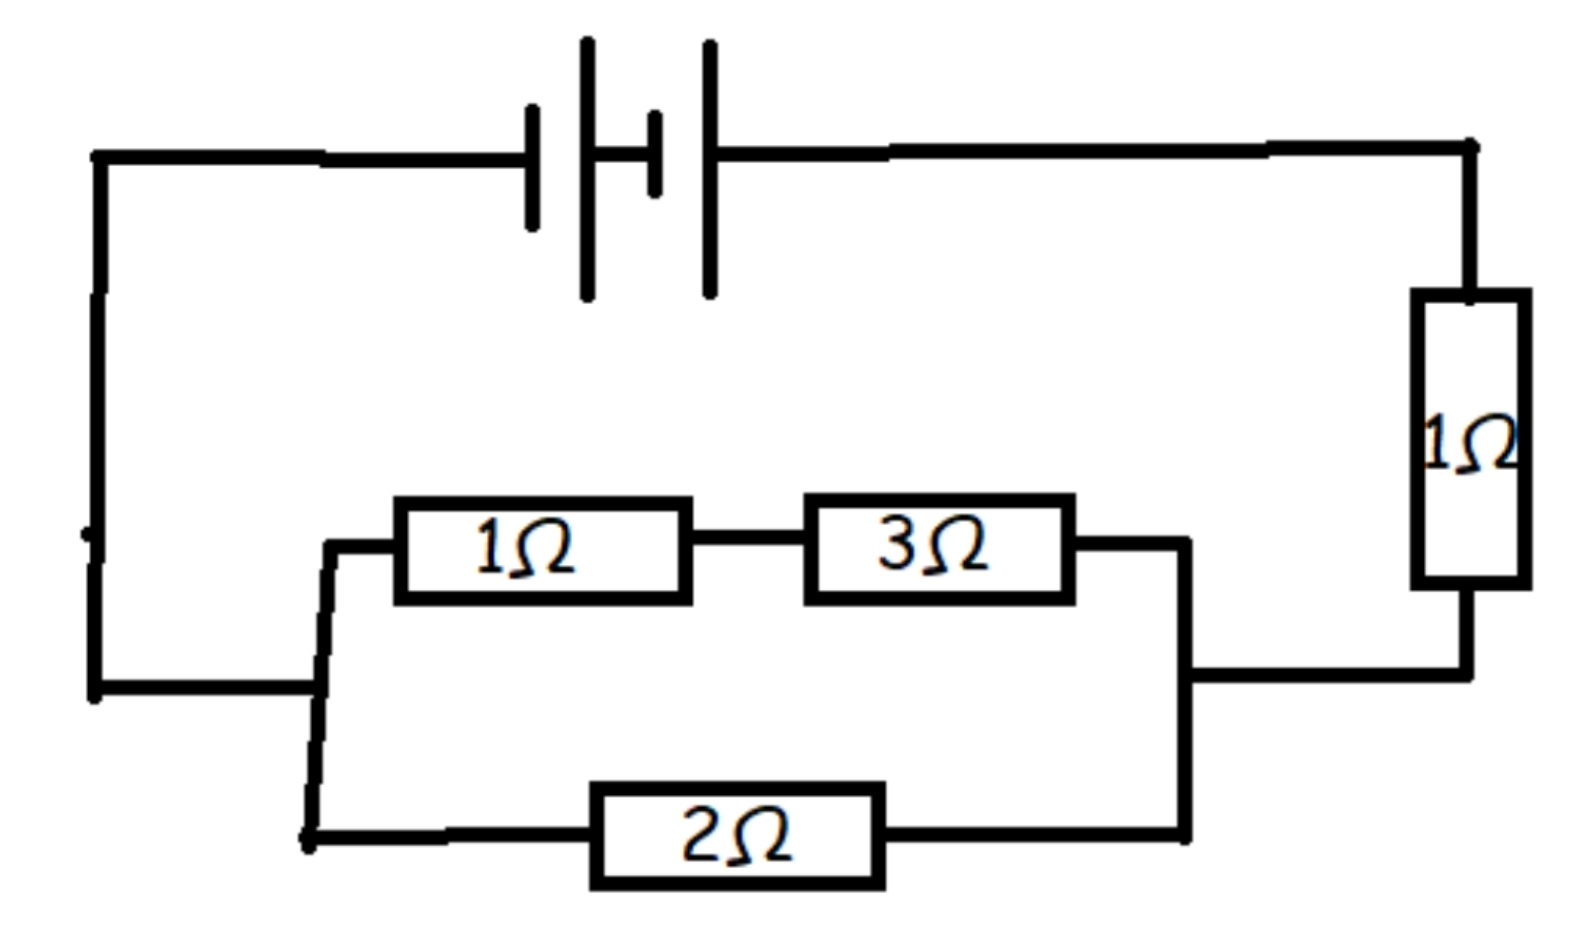
\includegraphics[height=4cm]{Electricity_Images/complex_circuit.jpg}
    \end{figure}

    The equivalent resistance of this circuit is: \pause 
    --2.3$\Omega$

    \begin{exampleblock}{Your Turn!}
        Now have a go at the Kerboodle examples on page 172!
    \end{exampleblock}
\end{frame}

\end{document}